\documentclass{article}
\usepackage[utf8]{inputenc}
\usepackage[margin=1.0in]{geometry}
\usepackage{graphicx}
\usepackage{wrapfig}
\usepackage{amsmath}
\usepackage[makeroom]{cancel}


\title{Edge Detection}
\author{Alexey Didenkov}
\date{October 24, 2018}

\begin{document}

\maketitle

\section{Introduction}
Images contain an enormous amount of information, with the majority of it being redundant. On the other hand, features such as edge points often carry important semantic information: contours of objects, creases, or shadow boundaries. Edge detection is one of the most important areas in lower computer vision, and it builds a foundation for many higher-level processing techniques. Edge points can be combined into continuous lines and contours, which are then used to identify objects in the scene. Edge points between different images can be used to recover depth information or detect moving objects. Likewise, edge detection appears to be a fundamental component in the human visual system - neurons responding to edges are present in the brain, and human infants can recognize scenes from just seeing their line drawings. 
\begin{figure}[!htb]
    \begin{center}
        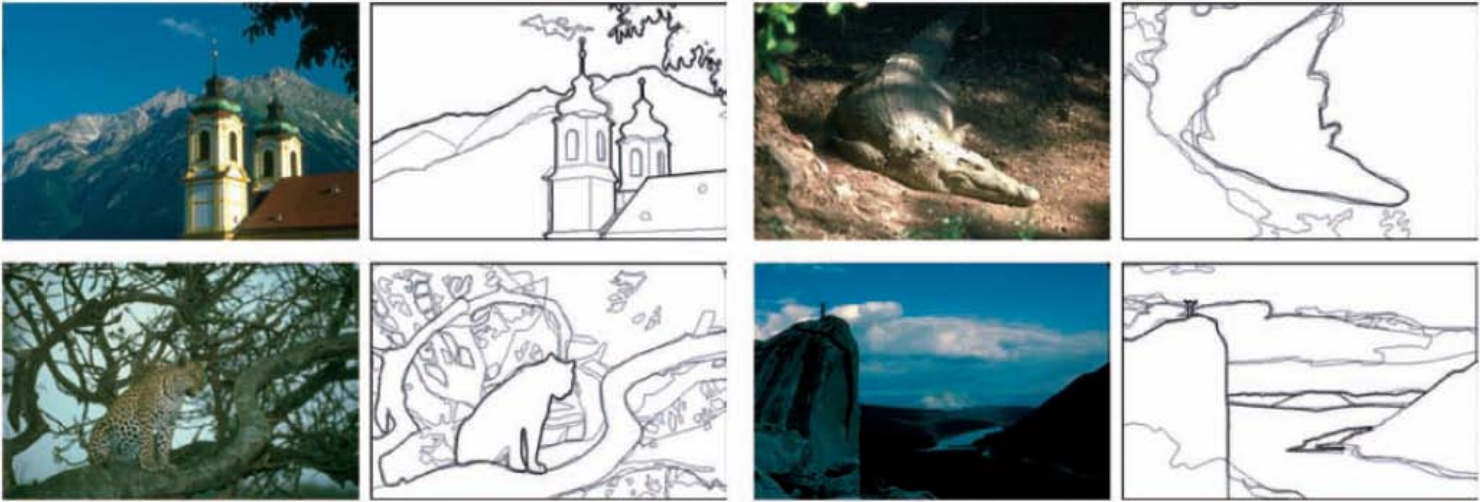
\includegraphics[width=0.8\textwidth]{Human_boundaries.png}
        \vspace{-10pt}
    \end{center}
    \caption{Human boundary detection (Martin, Fowlkes, and Malik 2004) © 2004 IEEE. The darkness of the edges corresponds to how many human subjects marked an object boundary at that location.}
\end{figure}

\section{Background}
\subsection{Image representation}
Real images are often represented with several channels of numerical values, where a value at a given pixel represents a specific feature of it, such as brightness, or the amount of the color red. While in the task of image segmentation we are interested in differences in color, intensity, or texture, for now let's put those under the abstract umbrella term \textbf{intensity} and treat our images as having a single channel of that intensity. In a real situation this intensity could be the grayscale value of an image, the average of the color channels, or the amount of presence of a certain texture.

\subsection{Convolutions}
A \textbf{convolution} is defined as shifting one function over the domain of another, and recording the area under the curve of their intersection:
\[( f * g ) ( t ) \stackrel { \mathrm { def } } { = } \int _ { - \infty } ^ { \infty } f ( \tau ) g ( t - \tau ) d \tau\]
This operation can be extended to two dimensions, with the main difference being that the function is now shifted over both dimensions.

For our purposes, however, we do not need to think of it so mathematically. Consider the two functions as two matrices, one being our image of intensity values, and the other a smaller in size matrix. Then, a convolution would involve placing that smaller matrix at every location on the image matrix and considering their overlap: multiplying the corresponding numbers and adding the products up.
\begin{figure}[!htb]
    \begin{center}
        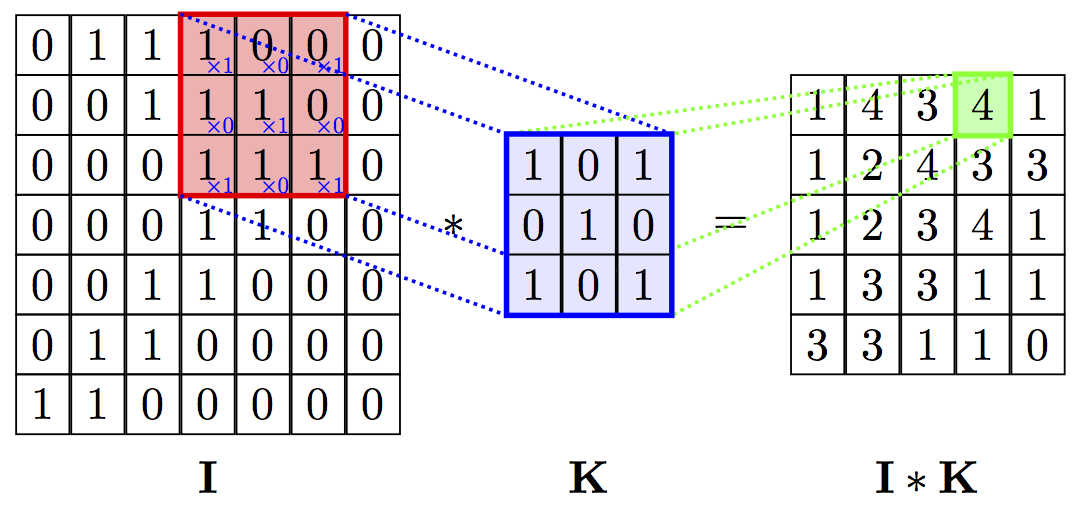
\includegraphics[width=0.8\textwidth]{2d_convolution.png}
        \vspace{-10pt}
    \end{center}
    \caption{A visual representation of 2D convolution}
\end{figure}

\section{Filtering}
Real images, especially ones with high resolution, often contain noise. While it disappears on a global scale, our edge detection algorithm will react to local noise unless we specifically average it out ourselves.
\subsection{Gaussian Filter}
The filter that we're looking for should consider a small neighborhood around each pixel and compute its average. Its neighborhood should look the same regardless of orientation, i.e. it should be circular. A popular choice is the \textbf{Gaussian filter}, which has a peak at its center and decreases with increase in radius. The Gaussian kernel is dependent on a parameter $\sigma$, which essentially controls its width. For center $(x _ { o }, y _ { o })$, widths $\sigma _ { x }$ and $\sigma _ { y }$, and peak altitude $A$, its formula is as follows:
\[f ( x , y ) = A \exp \left( - \frac { ( x - x _ { o } ) ^ { 2 } } { 2 \sigma _ { x } ^ { 2 } } - \frac { ( y - y _ { o } ) ^ { 2 } } { 2 \sigma _ { y } ^ { 2 } } \right)\]
For a curve with $\sigma _ { x } = \sigma _ { y } = \sigma$, center at $(0, 0)$, and volume under the curve of 1, the formula becomes:
\[f ( x , y ) = \frac { 1 } { 2 \pi \sigma ^ 2} \exp \left( - \frac { x ^ 2 + y ^ 2 } { 2 \sigma ^ { 2 } } \right)\]
Notice how the only term influenced by $x$ and $y$ can be reduced to $r^2=x^2+y^2$. This indicates that the Gaussian filter only depends on its radius from the origin and not the direction, making it circular and satisfying our aforementioned condition. When applied to an image, the Gaussian kernel has the effect of blurring it, with larger $\sigma$'s casing more blur.
\begin{figure}[!htb]
    \begin{center}
        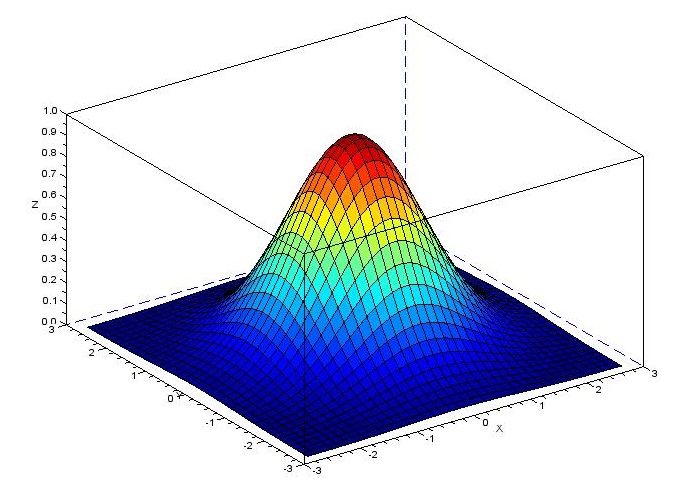
\includegraphics[width=0.45\textwidth]{gaussiankernel.jpg}
        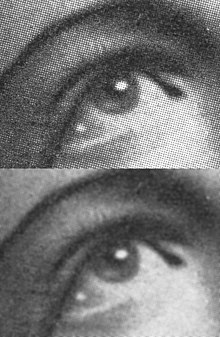
\includegraphics[width=0.2\textwidth]{blur.jpg}
    \end{center}
    \vspace{-10pt}
    \caption{The Gaussian filter and its effect}
\end{figure}
\subsection{Gaussian Kernel}
Since we need two matrices to perform a convolution, we need to turn the Gaussian filter function into a matrix, often called a \textbf{kernel}. To do this, we evaluate the continuous function at regular intervals, for all cells in the matrix. The result looks something like this:
\begin{figure}[!htb]
    \begin{center}
        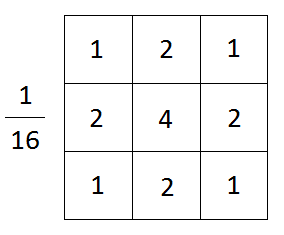
\includegraphics[width=0.25\textwidth]{gaussian3.png}
        \hspace{25pt}
        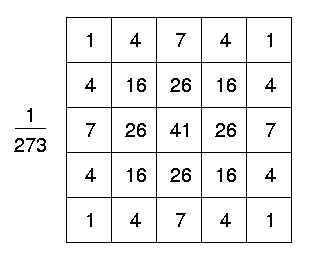
\includegraphics[width=0.25\textwidth]{gaussian5.png}
    \end{center}
    \vspace{-10pt}
    \caption{Gaussian kernels of two different sizes and $\sigma$'s}
\end{figure}
Notice the fraction in the front - we normalize the kernel's values so that they sum to 1 in order to guarantee the same range of values. Also notice how the size of the kernels is odd - this is often done to make centering the kernel on pixels easier. Similarly, sizes 7, 9, 11, and so forth are also quite popular, with larger sizes used in order to encompass kernels with larger $\sigma$'s, appropriate for images of larger resolutions\footnote{You can play around with the size and $\sigma$ parameters of Gaussian kernels here: http://dev.theomader.com/gaussian-kernel-calculator}. Keep in mind, through, that large kernels can slow down convolutions severely.

\section{Differentiation}
Qualitatively, edges occur at boundaries between regions of different intensity. Unfortunately, segmenting an image into coherent regions is a difficult task, so it is often preferable to detect edges using only purely local information. Let's define edges as regions of \textit{rapid intensity variation}, where the magnitude of edges reflects the steepness of the change.
\subsection{Sobel Kernel}
Now, we just need to find a kernel that reacts to edges in the aforementioned way. For now, let's just consider intensities varying with changes in $x$, i.e. vertical edges. This exact task can be done by a 1D kernel such as
\[\begin{bmatrix}
    -2 & 0 & 2 \\
\end{bmatrix}\]
On flat, constant regions, this kernel's left side will balance out its right side exactly. With sharp increases in intensity, its right side outweighs the left, and the result is positive. For decreases, the left side outweighs the right, and the result is negative.

We can easily extend this kernel to 2D, by adding similar but smaller rows above and below it:
\[\begin{bmatrix}
    -1 & 0 & 1 \\
    -2 & 0 & 2 \\
    -1 & 0 & 1 \\
\end{bmatrix}\]
This specific kernel is also called a \textbf{Sobel kernel}.
\subsection{Sobel Operator}
Since we're working with 2 dimensions, however, we now need to not only find increases to the right (positive-$x$), but also up (positive-$y$), up-right, up-up-right, and everything in-between. Fortunately, we aren't stuck checking an infinite amount of directions - it suffices to only apply the positive-$x$ and positive-$y$ kernels. These give us the \textit{x and y components} of the edge's direction. These are like the rectangular components of a vector, which we can use to find the direction and magnitude of the edge:
\[G = \sqrt {G_x^2 + G_y^2}\]
\[\theta = \cancel{ \operatorname{atan}(G_y / G_x) } = \operatorname{atan2}(G_y, G_x)\]
\begin{figure}[!htb]
    \begin{center}
        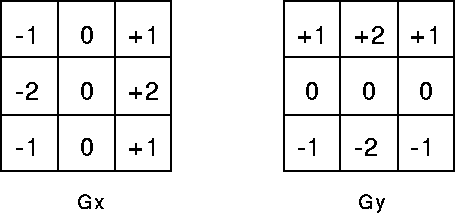
\includegraphics[width=0.4\textwidth]{sobelkernel.png}
        \hspace{20pt}
        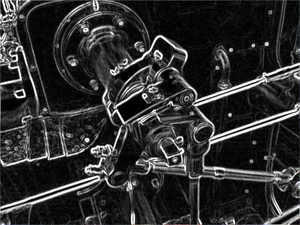
\includegraphics[width=0.285\textwidth]{outlines.PNG}
    \end{center}
    \vspace{-10pt}
    \caption{[left] The two fundamental Sobel kernels; [right] a processed image of Sobel magnitudes}
\end{figure}

\section{Edge thinning}
Simply applying the Sobel kernel often produces edges that are multiple pixels thick. This is often redundant information, as we are interested only in the centers of these thick edges and would often benefit from suppressing every other pixel. Also, we haven't used the edge direction information yet, and this is a way of incorporating it while eliminating redundancy.
\begin{figure}[!htb]
    \begin{center}
        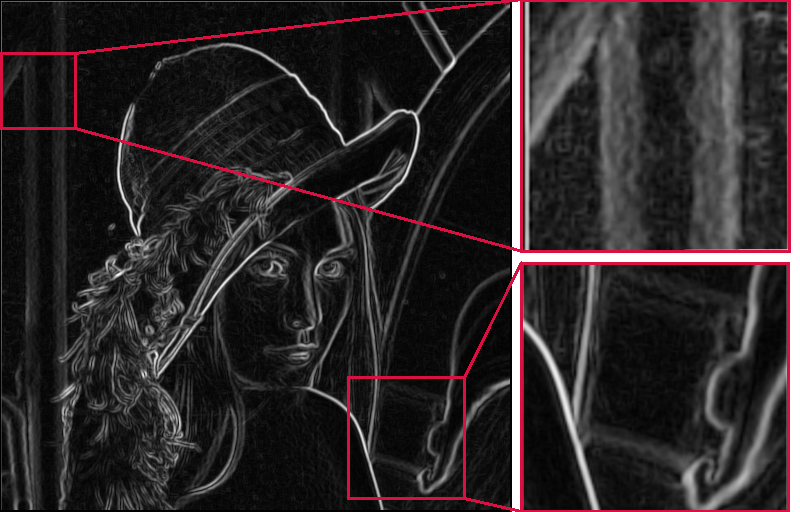
\includegraphics[width=0.35\textwidth]{lena_thick.png}
        \hspace{15pt}
        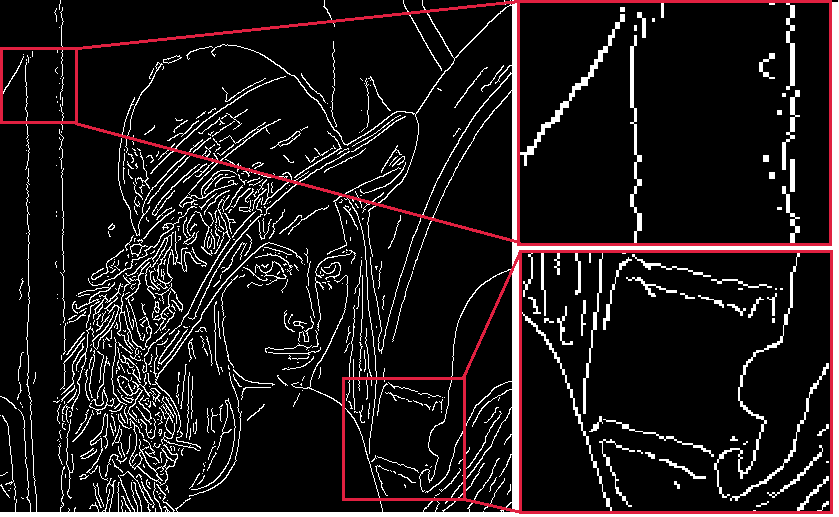
\includegraphics[width=0.365\textwidth]{lena_thin.png}
    \end{center}
    \vspace{-10pt}
    \caption{The result of a good edge thinning}
\end{figure}
\subsection{Non-maxima suppression}
The direction of the edge is the direction of greatest intensity change, and it is perpendicular to the contour line. Only keeping one pixel along the edge's direction ensures that variations are denoted by single edge pixels, while contours are continuous lines with the thickness of one pixel. We can choose this pixel by suppressing every other that isn't higher in magnitude than both of its directional neighbors.
\subsection{Thresholding}
Even with our edges thinned, there still remains plenty of redundant information between actual edges, mostly low-magnitude "edges" from small variations in background color. We can easily suppress these by only counting pixels that reach a certain \textbf{threshold}. We'll set the pixels that pass to 1, and those that fail to 0, essentially getting rid of magnitude, and only counting pixels as edges and non-edges.
\subsection{Hysteresis thresholding}
While trying delete enough background noise, we might end up needing to raise our threshold high enough for parts of actual edges to be erased. A simple way to avoid this is \textbf{hysteresis thresholding}, also known as \textbf{double-thresholding}. We now choose a min value and a max value, one about 3 times the other. Points below min value automatically fail, and points above max value automatically succeed. Points between the two thresholds only remain if they are part of an edge containing a pixel that is above max value. Such connections can be checked for with \textit{flood fill}.

\begin{wrapfigure}{r}{0.3\textwidth}
  \begin{center}
    \vspace{-20pt}
    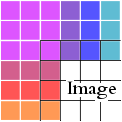
\includegraphics[width=0.20\textwidth]{Extend.png}
    \vspace{-17.5pt}
  \end{center}
  \caption{Extend edge behavior}
  \vspace{-50pt}
\end{wrapfigure}
\section{Edge behavior}
To perform convolutions, kernels sometimes need to be partially placed outside the image. There are several ways to resolve this:
\begin{itemize}
  \item \textbf{Crop}: Skip all such cases. Will result in the output image slightly shrinking in size.
  \item \textbf{Extend}: Repeat the last row/column of the image.
  \item \textbf{Mirror}: Append a reflection of the same border.
  \item \textbf{Wrap}: Append the opposing border of the image.
\end{itemize}

\section{Mathematical approach}
Previously, we had moved away from continuous functions in favor of using matrices and discrete convolutions. Now, let's return back to the fundamentals.
\subsection{Background}
Most of the math here relies on multivariable calculus, so here are some of the main ideas needed to understand what's going on:

Here, we consider functions of two independent variables, $f(x, y)$. You can visualize them in 3 dimensions, with the output value on the z-axis.

The \textbf{gradient} of $f$ is denoted as $\nabla f$, and it is somewhat analogous to the derivative. It takes in scalar values and returns vectors that point in the direction of steepest increase, with their magnitudes reflecting the amount of increase. It is found like so:
\[\nabla f = \operatorname { grad } f = \langle \frac { \partial f } { \partial x }, \frac { \partial f } { \partial y }, \frac { \partial f } { \partial z } \rangle \]

The \textbf{divergence} of $\vec v$ is denoted as $\nabla \cdot \vec v$. It takes in a \textbf{vector field} $\vec v$ (multiple vectors in continuous coordinates) and returns scalars that roughly represent the vector field's increase in the direction of the vector at a given point. It is found like so:
\[\nabla \cdot \vec { v } = \operatorname { div } \vec { v } = \frac { \partial v _ { x } } { \partial x } + \frac { \partial v _ { y } } { \partial y } + \frac { \partial v _ { z } } { \partial z }\]

\subsection{Laplacian of Gaussian}
If we think of images as a height fields of intensity values, their edges become represented by \textit{steep slopes} on the surface, which can be found through the surface's gradient:
\[J( \boldsymbol { x } ) = \nabla I( \boldsymbol { x } ) = \langle\frac{\partial I}{\partial x}, \frac{\partial I}{\partial y}\rangle( \boldsymbol { x } )\]
The local gradient vector \textbf{J} points in the direction of \textit{steepest ascent} in the intensity function. Its magnitude indicates the slope or strength of the variation, while its orientation
points in a direction perpendicular to the local contour.

The gradient \textit{after applying the Gaussian kernel} then becomes
\[J _ { \sigma }( \boldsymbol { x } ) = \nabla \left[ G _ { \sigma }( \boldsymbol { x } ) * I ( \boldsymbol { x } )\right] = \left[ \nabla G _ { \sigma } \right]( \boldsymbol { x } ) * I( \boldsymbol { x } )\]
\[\nabla G _ { \sigma }( \boldsymbol { x } ) = \langle \frac { \partial G _ { \sigma } } { \partial x } , \frac { \partial G _ { \sigma } } { \partial y } \rangle( \boldsymbol { x } ) = -\frac { 1 } { 2 \pi \sigma ^ { 4 } } \exp \left( - \frac { x ^ { 2 } + y ^ { 2 } } { 2 \sigma ^ { 2 } } \right)\langle x, y \rangle\]

\begin{wrapfigure}{r}{0.25\textwidth}
  \begin{center}
    \vspace{-30pt}
    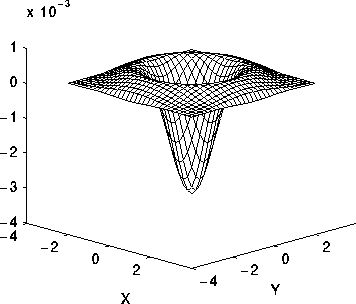
\includegraphics[width=0.22\textwidth]{log.png}
    \vspace{-17.5pt}
  \end{center}
  \caption{LoG kernel}
  \vspace{-0pt}
\end{wrapfigure}
To perform edge-thinning, we can consider the divergence of our gradient of the Gaussian of the image. This divergence will examine magnitudes of edges along the directions of the edges, just like we did previously. As the magnitude stops increasing and starts decreasing, divergence goes from positive to negative and crosses zero - that's our clue of where to find edges.
\[S _ { \sigma } ( \boldsymbol { x } ) = \nabla \cdot \boldsymbol { J } _ { \sigma } ( \boldsymbol { x } ) = \left[ \nabla ^ { 2 } G _ { \sigma } \right] ( \boldsymbol { x } ) * I ( \boldsymbol { x } )\]
\[\nabla ^ { 2 } G _ { \sigma } ( \boldsymbol { x } ) = -\frac { 1 } { 2 \pi \sigma ^ { 4 } } \left( 2 - \frac { x ^ { 2 } + y ^ { 2 } } { 2 \sigma ^ { 2 } } \right) \exp \left( - \frac { x ^ { 2 } + y ^ { 2 } } { 2 \sigma ^ { 2 } } \right) = -\frac { 1 } { \sigma ^ { 2 } } \left( 2 - \frac { x ^ { 2 } + y ^ { 2 } } { 2 \sigma ^ { 2 } } \right) G _ { \sigma } ( \boldsymbol { x } )\]

Note that the final result is a convolution of the second order gradient of the Gaussian with the original image. We thus call the convolution \textbf{Laplacian of Gaussian}, and the second order gradient the \textbf{LoG kernel}.

\section{Extensions}
Today, we looked at a process called \textbf{Canny edge detection}, which used the \textit{Sobel kernel}, and then derived the \textit{LoG kernel}. There exist many more kernels to find edges (\textit{Prewit, Robert's, Haralick}, etc.). There are kernels that focus on slightly different goals, kernels whose convolution can be optimized, kernels that define edges differently, kernels inspired by the visual system. All of them are unique in their performances.

\section{Applications}
Today we left off with finding edge pixels. Knowing that these define contours, we can proceed to link these pixels together into edges, and edges together into contours and regions through \textbf{edge linking}. We can use \textit{curve smoothing} to eliminate noise and produce nicer edges. We can utilize \textbf{Hough transform} if looking for straight lines or circles. Parallel lines in the scene can then be used to undistort textures through \textbf{perspective correction} or to infer structure or depth. \textbf{Region segmentation} can be extensively used to detect objects or to attempt \textbf{scene understanding}.

\end{document}